%! suppress = MissingImport
The columns marked with red and blue stripes are the power bus strips, also known as the power rails.
You will now provide power to the bus strips so that the other components can use power.

\disconnect\

Take the \rainbow, and peel off two wires.
Insert one end of a wire into contact point \mcufivevoltcontactpoint\ (notice that contact point \mcufivevoltcontactpoint\ is electrically connected to the \developmentboard's \texttt{5V} pin, which is in contact point \mcufivevolt).
Insert the other end of the \texttt{5V} wire into the upper \power\ marked with a red stripe.
Now insert one end of the other wire into contact point \mcuuppergroundcontactpoint\ (notice that contact point \mcuuppergroundcontactpoint\ is electrically connected to one of the \developmentboard's \texttt{GND} pins, which is in contact point \mcuuppergroundcontactpoint).
Insert the other end of the \texttt{GND} wire into the upper \ground\ marked with a blue stripe.
See Figure~\ref{fig:power-without-template}.
If you are using a breadboard template, you will need to fold back the paper (or cut away some paper) to access the power rails;
see Figure~\ref{fig:power-with-template}.

\begin{figure}
    \centering
    \subfloat[Tapping power and ground from the \developmentboard.]{
        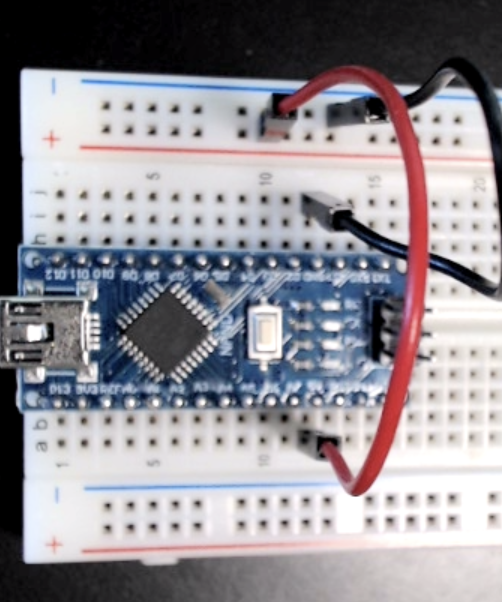
\includegraphics[width=0.4\textwidth]{direct/power/power-without-template}
        \label{fig:power-without-template}
    }
    \hfil
    \subfloat[Tapping power and ground from the \developmentboard\ when using a breadboard template.]{
        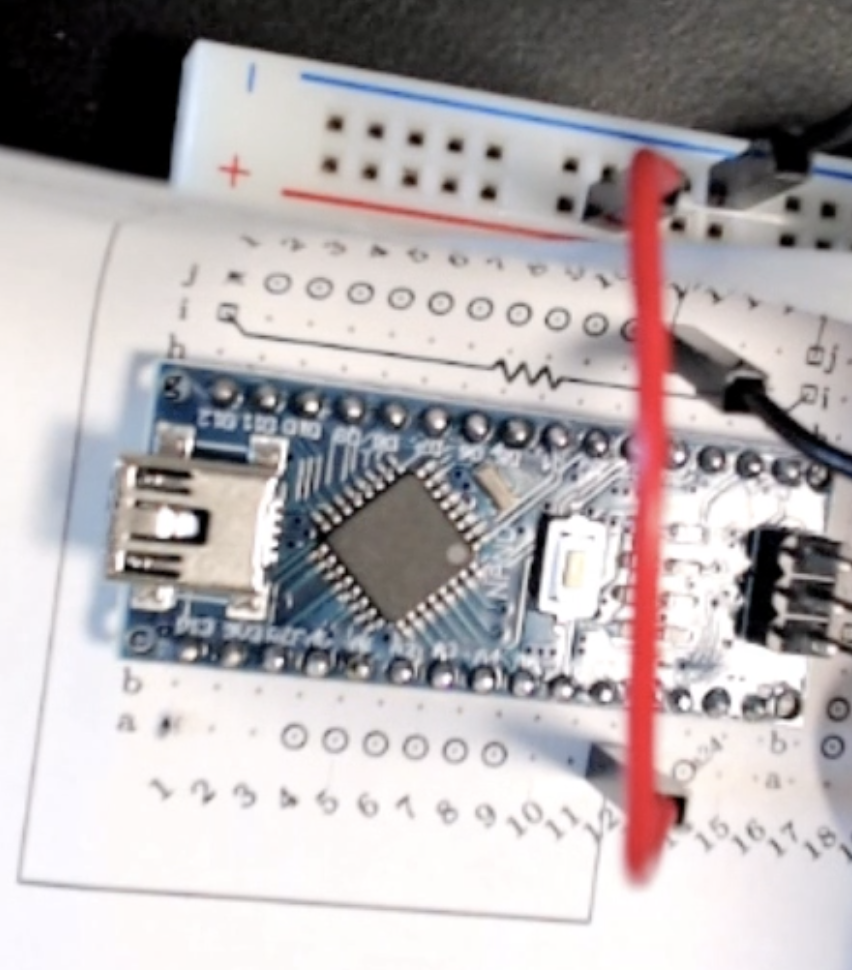
\includegraphics[width=0.4\textwidth]{direct/power/power-with-template}
        \label{fig:power-with-template}
    }
    \caption{Providing power and ground to power busses.}
\end{figure}

\checkpoint{connected the \developmentboard\ to the upper \power\ and the upper \ground}
